\section*{2. Probability}\label{probability}

\subsection*{2.2 Sample Spaces and Events}\label{sample-spaces-and-events}

The \textbf{sample space} \(\Omega\) is the set of possible outcomes of an experiment. Points \(\omega\) in \(\Omega\) are called \textbf{sample outcomes} or \textbf{realizations}. \textbf{Events} are subsets of \(\Omega\).

Given an event \(A\), let \(A^{c} = \{ \omega \in \Omega : \text{not } (\omega \in A) \}\) denote the complement of \(A\). The complement of \(\Omega\) is the empty set \(\varnothing\). The union of events \(A\) and \(B\) is defined as \(A \cup B = \{ \omega \in \Omega : \omega \in A \text{ or } \omega \in B \}\). If \(A_{1}, A_{2}, \dots\) is a sequence of sets, then

\[ 
\cup_{i=1}^{\infty} A_{i} = \left\{ \omega \in \Omega : \omega \in A_{i} \text{ for some } i \right\}
\]

The intersection of \(A\) and \(B\) is 
\(A \cap B = \{ \omega \in \Omega : \omega \in A \text{ and } \omega \in B \}\).
If \(A_{1}, A_{2}, \dots\) is a sequence of sets then

\[ 
\cap_{i=1}^{\infty} A_{i} = \left\{ \omega \in \Omega : \omega \in A_{i} \text{ for all } i \right\}
\]

Let
\(A - B = \left\{ \omega \in \Omega : \omega \in A \text{ and not } (\omega \in B) \right\}\).
If every element of \(A\) is contained in \(B\) we write \(A \subset B\) or \(B \supset A\). If \(A\) is a finite set, let \(|A|\) denote the number of elements in \(A\).

\begin{table}[H]
\centering
\begin{tabular}{@{}p{5cm}p{10cm}@{}}
\toprule
notation &  meaning  \\
\midrule
\(\Omega\) & sample space \\
\(\omega\) & outcome \\
\(A\) & event (subset of \(\Omega\)) \\
\(\vert A \vert\) & number of elements in \(A\) (if finite) \\
\(A^{c}\) & complement of \(A\) (not \(A\)) \\
\(A \cup B\) & union (\(A\) or \(B\)) \\
\(A \cap B\) or \(AB\) & intersection (\(A\) and \(B\)) \\
\(A - B\) & set difference (points in \(A\) but not in \(B\)) \\
\(A \subset B\) & set inclusion (\(A\) is a subset of or equal to
\(B\)) \\
\(\varnothing\) & null event (always false) \\
\(\Omega\) & true event (always true) \\
\bottomrule
\end{tabular}
\end{table}

We say that \(A_{1}, A_{2}, \dots\) are \textbf{disjoint} or \textbf{mutually exclusive} if \(A_{i} \cap A_{j} = \varnothing\) whenever \(i \neq j\). A \textbf{partition} of \(\Omega\) is a sequence of disjoint sets \(A_{1}, A_{2}, \dots\) such that \(\cup_{i=1}^{\infty} A_{i} = \Omega\). Given an event \(A\), define the \textbf{indicator function of \(A\)} by

\[ 
I_A(\omega) = I(\omega \in A) = 
\begin{cases}
1 &\text{if } \omega \in A 
\\
0 &\text{otherwise}
\end{cases}
\]

A sequence of sets \(A_{1}, A_{2}, \dots\) is \textbf{monotone increasing}
if \(A_{1} \subset A_{2} \subset \dots\), and we define \(\lim_{n \rightarrow \infty} A_{n} = \cup_{i=1}^{\infty} A_{i}\). A sequence of sets \(A_{1}, A_{2}, \dots\) is \textbf{monotone decreasing} if \(A_{1} \supset A_{2} \supset \dots\) and then we define \(\lim_{n \rightarrow \infty} A_{n} = \cap_{i=1}^{n} A_{i}\). In either case, we will write \(A_{n} \rightarrow A\).

\subsection*{2.3 Probability}

A function \(\mathbb{P}\) that assign a real number \(\mathbb{P}(A)\) to each event \(A\) is a \textbf{probability distribution} or a \textbf{probability measure} if it satisfies the following three axioms:

\begin{itemize}[tightlist]
\item
  \textbf{Axiom 1}: \(\mathbb{P}(A) \geq 0\) for every \(A\)
\item
  \textbf{Axiom 2}: \(\mathbb{P}(\Omega) = 1\)
\item
  \textbf{Axiom 3}: If \(A_{1}, A_{2}, \dots\) are disjoint then
\end{itemize}

\[ \mathbb{P} \left( \cup_{i=1}^{\infty} A_{i} \right) = \sum_{i=1}^{\infty} \mathbb{P}(A_{i}) \]

A few properties that can be derived from the axioms:

\begin{itemize}[tightlist]
\item
  \(\mathbb{P}(\varnothing) = 0\)
\item
  \(A \subset B \Rightarrow \mathbb{P}(A) \leq \mathbb{P}(B)\)
\item
  \(0 \leq \mathbb{P}(A) \leq 1\)
\item
  \(\mathbb{P}\left(A^{c}\right) = 1 - \mathbb{P}(A)\)
\item
  \(A \cap B = \varnothing \Rightarrow \mathbb{P}(A \cup B) = \mathbb{P}(A) + \mathbb{P}(B)\)
\end{itemize}

\textbf{Lemma 2.6}. For any events \(A\) and \(B\),
\(\mathbb{P}(A \cup B) = \mathbb{P}(A) + \mathbb(B) - \mathbb{P}(AB)\).

\textbf{Proof}.

\begin{align*}
\mathbb{P}(A \cup B) 
&= \mathbb{P}\left( (AB^{c}) \cup (AB) \cup (A^{c}B) \right) 
\\
&= \mathbb{P}(AB^{c}) + \mathbb{P}(AB) + \mathbb{P}(A^{c}B) 
\\
&= \mathbb{P}(AB^{c}) + \mathbb{P}(AB) + \mathbb{P}(A^{c}B) + \mathbb{P}(AB) - \mathbb{P}(AB) 
\\
&= \mathbb{P}((AB^{c}) \cup (AB)) + \mathbb{P}((A^{c}B) \cup (AB)) - \mathbb{P}(AB) 
\\
&= \mathbb{P}(A) + \mathbb{P}(B) - \mathbb{P}(AB)
\end{align*}

\textbf{Theorem 2.8 (Continuity of Probabilities)}. If
\(A_{n} \rightarrow A\) then \(\mathbb{P}(A_{n}) \rightarrow \mathbb{P}(A)\)
as \(n \rightarrow \infty\).

\textbf{Proof}. Suppose that \(A_{n}\) is monotone increasing,
\(A_{1} \subset A_{2} \subset \dots\). Let \(B_{1} = A_{1}\), and
\(B_{n+1} = A_{n+1} - A_{n}\) for \(n > 1\). The \(B_{i}\)s are disjoint by
construction, and \(A_{n} = \cup_{i=1}^{n} A_{i} = \cup_{i=1}^{n} B_{i}\) for all
\(n\). From axiom 3,

\[ \mathbb{P}(A_{n}) = \mathbb{P}\left( \cup_{i=1}^{n} B_{i} \right)  = \sum_{i=1}^{n} \mathbb{P}(B_{i}) \]

and so

\[ \lim_{n \rightarrow \infty} \mathbb{P}(A_{n}) = \lim_{n \rightarrow \infty} \sum_{i=1}^{n} \mathbb{P}(B_{n}) = \sum_{i=1}^{\infty} \mathbb{P}(B_{n}) = \mathbb{P}\left( \cup_{i=1}^{\infty} B_{i} \right) = \mathbb{P}(A) \]

\subsection*{2.4 Probability on Finite Sample Spaces}\label{probability:samples}

If \(\Omega\) is finite and each outcome is equally likely, then

\[ \mathbb{P}(A) = \frac{|A|}{|\Omega|} \]

which is called the \textbf{uniform probability distribution}.

We will need a few facts from counting theory later.

\begin{itemize}
\item
  Given \(n\) objects, the number of way or ordering these objects is
  \(n! = n \cdot (n - 1) \cdot (n - 2) \cdots 3 \cdot 2 \cdot 1\). We
  define \(0! = 1\).
\item
  We define

  \[ \binom{n}{k} = \frac{n!}{k! (n - k)!} \]

  read ``n choose k'', which is the number of different ways of choosing
  \(k\) objects from \(n\).
\item
  Note that choosing a subset \(k\) objects can be mapped to choosing
  the complement set of \(n - k\) objects, so

  \[ \binom{n}{k} = \binom{n}{n - k} \]

  and that there is only one way of choosing the empty set, so

  \[ \binom{n}{0} = \binom{n}{n} = 1\]
\end{itemize}

\subsection*{2.5 Independent Events}\label{independent:events}

\begin{itemize}
\item
  Two events \(A\) and \(B\) are \textbf{independent} if

  \[ \mathbb{P}(AB) = \mathbb{P}(A) \, \mathbb{P}(B) \]

  and we write \(A \text{ ⫫ } B\). A set of events
  \(\{ A_{i} : i \in I \}\) is independent if

  \[ \mathbb{P} \left( \cap_{i \in J} A_{i} \right) = \prod_{i \in J} \mathbb{P}(A_{i}) \]

  for every finite subset \(J\) of \(I\).
\item
  Independence is sometimes assumed and sometimes derived.
\item
  Disjoint events with positive probability are not independent.
\end{itemize}

\subsection*{2.6 Conditional Probability}\label{conditional-probability}

\begin{itemize}
\item
  If \(\mathbb{P}(B) > 0\) then the \textbf{conditional probability} of
  \(A\) given \(B\) is

  \[ \mathbb{P}(A | B) = \frac{\mathbb{P}(AB)}{\mathbb{P}(B)} \]
\item
  \(\mathbb{P}(\cdot | B)\) satisfies the axioms of probability, for
  fixed \(B\). 
\item 
  In general, \(\mathbb{P}(A | \cdot)\) does \textbf{not}
  satisfies the axioms of probability for fixed \(A\).
\item
  In general, \(\mathbb{P}(B | A) \neq \mathbb{P}(A | B)\).
\item
  \(A\) and \(B\) are independent if and only if
  \(\mathbb{P}(A | B) = \mathbb{P}(A)\).
\end{itemize}

\subsection*{2.7 Bayes' Theorem}\label{bayes:theorem}

\textbf{Theorem 2.15 (The Law of Total Probability)}. Let
\(A_{1}, \dots, A_{k}\) be a partition of \(\Omega\). Then, for any event
\(B\),

\[ 
\mathbb{P}(B) 
= \sum_{i=1}^{k} \mathbb{P}(B | A_{i}) \, \mathbb{P}(A_{i}) 
\]

\textbf{Proof}. Let \(C_{j} = BA_{j}\). Note that the \(C_{j}\)s are disjoint
and that \(B = \cup_{i=1}^{k} C_{j}\). Hence

\[ 
\mathbb{P}(B) 
= \sum_{j} \mathbb{P}(C_{j})  
= \sum_{j} \mathbb{P}(BA_{j}) 
= \sum_{j} \mathbb{P}(B | A_{j}) \, \mathbb{P}(A_{j}) 
\]

\textbf{Theorem 2.16 (Bayes' Theorem)}. Let \(A_{1}, \dots, A_{k}\) be a
partition of \(\Omega\) such that \(\mathbb{P}(A_{i}) > 0\) for each
\(i\). If \(\mathbb{P}(B) > 0\), then, for each \(i = 1, \dots, k\),

\[ 
\mathbb{P}(A_{i} | B) = \frac{\mathbb{P}(B | A_{i}) \, \mathbb{P}(A_{i})}{\sum_{j} \mathbb{P}(B | A_{j}) \, \mathbb{P}(A_{j})} 
\]

We call \(\mathbb{P}(A_{i})\) the \textbf{prior probability} of \(A_{i}\)
and \(\mathbb{P}(A_{i} | B)\) the \textbf{posterior probability} of
\(A_{i}\).

\textbf{Proof}. We apply the definition of conditional probability
twice, followed by the law of total probability:

\[ 
\mathbb{P}(A_{i} | B) 
= \frac{\mathbb{P}(A_{i} B) }{\mathbb{P}(B)} 
= \frac{\mathbb{P}(B | A_{i}) \, \mathbb{P}(A_{i})}{\mathbb{P}(B)} 
= \frac{\mathbb{P}(B | A_{i}) \, \mathbb{P}(A_{i})}{\sum_{j} \mathbb{P}(B | A_{j}) \, \mathbb{P}(A_{j})}
\]

\subsection*{2.9 Technical Appendix}

Generally, it is not feasible to assign probabilities to all the subsets of a sample space \(\Omega\). Instead, one restricts attention to a set of events called a \textbf{\(\sigma\)-algebra} or a \textbf{\(\sigma\)-field}, which is a class \(\mathcal{A}\) that satisfies:

\begin{itemize}[tightlist]
\item
  \(\varnothing \in \mathcal{A}\)
\item
  If \(A_{1}, A_{2}, \dots \in \mathcal{A}\), then
  \(\cup_{i=1}^{\infty} A_{i} \in \mathcal{A}\)
\item
  \(A \in \mathcal{A}\) implies that \(A^{c} \in \mathcal{A}\)
\end{itemize}

The sets in \(\mathcal{A}\) are said to be \textbf{measurable}. We call \((\Omega, \mathcal{A})\) a \textbf{measurable space}. If \(\mathbb{P}\) is a probability measure defined in \(\mathcal{A}\) then \((\Omega, \mathcal{A}, \mathbb{P})\) is a \textbf{probability space}. When \(\Omega\) is the real line, we take \(\mathcal{A}\) to be the smallest \(\sigma\)-field that contains all off the open sets, which is called the \textbf{Borel \(\sigma\)-field}.

\subsection*{2.10 Exercises}

\textbf{Exercise 2.10.1}. Fill in the details in the proof of Theorem~2.8. Also, prove the monotone decreasing case.

If \(A_{n} \rightarrow A\) then \(\mathbb{P}(A_{n}) \rightarrow \mathbb{P}(A)\) as \(n \rightarrow \infty\).

\textbf{Solution}.

Suppose that \(A_{n}\) is monotone increasing, \(A_{1} \subset A_{2} \subset \dots\). Let \(B_{1} = A_{1}\), and \(B_{i+1} = A_{i+1} - A_{i}\) for \(i > 1\).

The \(B_{i}\)s are disjoint by construction: assuming without loss of generality \(i < j\), \(\omega \in B_{i} \cap B_{j}\) implies that \(\omega\) is in \(A_{j}\), \(A_{i}\), but not in \(A_{j - 1}\), \(A_{i - 1}\), where \(A_{0} = \varnothing\). In particular, this means that \(\omega \in A_{i}\) but not \(\omega \in A_{j - 1}\). Since \(A_{i} \subset A_{j - 1}\), this implies that no such \(\omega\) can satisfy those properties, and so \(B_{i}\) and \(B_{j}\) are disjoint.

Note that \(A_{n} = \cup_{i=1}^{n} A_{i} = \cup_{i=1}^{n} B_{i}\) for all \(n\):

\[ \cup_{i=1}^{n} B_{i} = \cup_{i=1}^{n} (A_{i} - A_{i - 1}) \subset \cup_{i=1}^{n} A_{i} = A_{n} \]

Also note that \(A_{n} \subset \cup_{i=1}^{n} B_{i}\), since, if
 \(f(\omega) = \min \{ k : \omega \in A_{k} \}\), then \(\omega \in B_{f(\omega)}\), so all elements of \(A_{n}\) are in some \(B_{k}\).

The proof follows from Axiom 3,

\[ \mathbb{P}(A_{n}) = \mathbb{P}\left( \cup_{i=1}^{n} B_{i} \right) = \sum_{i=1}^{n} \mathbb{P}(B_{i}) \]

and so

\[ \lim_{n \rightarrow \infty} \mathbb{P}(A_{n}) = \lim_{n \rightarrow \infty} \sum_{i=1}^{n} \mathbb{P}(B_{n}) = \sum_{i=1}^{\infty} \mathbb{P}(B_{n}) = \mathbb{P}\left( \cup_{i=1}^{\infty} B_{i} \right) = \mathbb{P}(A) \]

The monotone decreasing case can be obtained by looking at the complementary series \(A_{1}^{c}, A_{2}^{c}, \dots\),which is monotone increasing. We get

\begin{align*}
\lim_{n \rightarrow \infty} \mathbb{P}(A_{n}^{c}) 
&= \mathbb{P}(A^{c}) 
\\
\lim_{n \rightarrow \infty} 1 - \mathbb{P}(A_{n}^{c}) 
&= 1 - \mathbb{P}(A^{c}) 
\\
\lim_{n \rightarrow \infty} \mathbb{P}(A_{n}) 
&= \mathbb{P}(A)
\end{align*}

\textbf{Exercise 2.10.2}. Prove the statements in equation (2.1).

\begin{itemize}[tightlist]
\item
  \(\mathbb{P}(\varnothing) = 0\)
\item
  \(A \subset B \Rightarrow \mathbb{P}(A) \leq \mathbb{P}(B)\)
\item
  \(0 \leq \mathbb{P}(A) \leq 1\)
\item
  \(\mathbb{P}\left(A^{c}\right) = 1 - \mathbb{P}(A)\)
\item
  \(A \cap B = \varnothing \Rightarrow \mathbb{P}(A \cup B) = \mathbb{P}(A) + \mathbb{P}(B)\)
\end{itemize}

\textbf{Solution}.

\begin{itemize}
\item
  By partitioning the event space \(\Omega\) into disjoint partitions
  \((\Omega, \varnothing)\) we get

  \[ \mathbb{P}(\Omega) + \mathbb{P}(\varnothing) = \mathbb{P}(\Omega) \Rightarrow \mathbb{P}(\varnothing) = 0 \]
\item
  Assuming \(A \subset B\) and partitioning \(B\) as \((A, B - A)\), we
  get

  \[ \mathbb{P}(A) + \mathbb{P}(B - A) = \mathbb{P}(B) \Rightarrow \mathbb{P}(A) \leq \mathbb{P}(B) \]
\item
  \(\mathbb{P}(A) \geq 0\) from axiom 1. By partitioning \(\Omega\) as
  \((A, A^{c})\), we get

  \[ \mathbb{P}(A) + \mathbb{P}(A^{c}) = \mathbb{P}(\Omega) = 1 \Rightarrow \mathbb{P}(A) \leq 1 \]
\item
  By partitioning \(\Omega\) as \((A, A^{c})\), we get

  \[ \mathbb{P}(A) + \mathbb{P}(A^{c}) = \mathbb{P}(\Omega) = 1 \Rightarrow \mathbb{P}(A) = 1 - \mathbb{P}(A^{c}) \]
\item
  Assuming \(A\), \(B\) are disjoint, we partition \(A \cup B\) in
  \((A, B)\) and get:

  \[ \mathbb{P}(A \cup B) = \mathbb{P}(A) + \mathbb{P}(B) \]
\end{itemize}

\textbf{Exercise 2.10.3}. Let \(\Omega\) be a sample space and let
\(A_{1}, A_{2}, \dots\) be events. Define \(B_{n} = \cup_{i=n}^{\infty} A_{i}\)
and \(C_{n} = \cap_{i=n}^{\infty} A_{i}\)

\textbf{(a)} Show that \(B_{1} \supset B_{2} \supset \cdots\) and
\(C_{1} \subset C_{2} \subset \cdots\).

\textbf{(b)} Show that \(\omega \in \cap_{n = 1}^{\infty} B_{n}\) if and
only if \(\omega\) belongs to an infinite number of the events
\(A_{1}, A_{2}, \dots\).

\textbf{(c)} Show that \(\omega \in \cup_{n = 1}^{\infty} C_{n}\) if and
only if \(\omega\) belongs to all of the events \(A_{1}, A_{2}, \dots\)
except possibly a finite number of those events.

\textbf{Solution}.

\textbf{(a)} By construction, \(B_{n+1} = A_{n} \cup B_{n}\) and so
\(B_{n + 1} \supset B_{n}\). Similarly, \(C_{n+1} = A_{n} \cap C_{n}\) and so
\(C_{n + 1} \subset C_{n}\).

\textbf{(b)}

\begin{itemize}
\item
  Assume \(\omega\) belongs to an infinite number of the events,
  \(\omega \in A_{j}\) for \(j \in J(\omega)\). Then, for every \(n\),
  there is a \(m \geq n\) such that \(m \in J(\omega)\), and so
  \(\omega \in B_{n}\) for every \(n\). This implies that
  \(\omega \in \cap_{n = 1}^{\infty} B_{n}\).
\item
  Assume that \(\omega \in \cap_{n = 1}^{\infty} B_{n}\). Then, for every
  \(n\), \(\omega \in B_{n}\), so for every \(n\) there is a \(m \geq n\)
  such that \(\omega \in A_m\). This implies there is an infinite number
  of such events \(A_m\).
\end{itemize}

\textbf{(c)}

Prove the contrapositive.

\begin{itemize}[tightlist]
\item
  Assume that \(\omega\) does not belong to an infinite number of events
  \(A_{i}\). Then, for every \(n\), there is a \(m \geq\) such that
  \(\omega \in A_m^{c}\), and so \(\omega\) is not in \(C_{n}\). Since
  \(\omega\) is not in none of the \(C_{n}\)s, it is not in the union of
  all \(C_{n}\)s either.
\item
  Assume that \(\omega\) is not in the union of all \(C_{n}\). This
  implies that \(\omega\) is is not in any event \(C_{n}\). This implies
  that, for every \(n\), there is a \(m \geq n\) such that \(\omega\) is
  not in \(A_m\). This implies that there is an infinite number of such
  events \(A_m\).
\end{itemize}

\textbf{Exercise 2.10.4}. Let \(\{ A_{i} : i \in I \}\) be a collection of
events where \(I\) is an arbitrary index set. Show that

\[ \
\left( \cup_{i \in I} A_{i} \right)^{c} = \cap_{i \in I} A_{i}^{c} 
\quad \text{and} \quad
\left( \cap_{i \in I} A_{i} \right)^{c} = \cup_{i \in I} A_{i}^{c} 
\]

Hint: First prove this for \(I = \{1, \dots, n\}\).

\textbf{Solution}.

We can prove the result directly by noting that every outcome \(\omega\) belongs to or does not belong to both sides of each equality:

\begin{align*}
& \omega \in \left( \cup_{i \in I} A_{i} \right)^{c} 
\\
\Longleftrightarrow
& \; \text{not }\left( \omega \in \cup_{i \in I} A_{i}  \right) 
\\
\Longleftrightarrow
& \; \forall i \in I, \text{not} \left( \omega \in A_{i} \right) 
\\
\Longleftrightarrow
& \; \forall i \in I, \omega \in A_{i}^{c} 
\\
\Longleftrightarrow
& \; \omega \in \cap_{i \in I} A_{i}^{c}
\end{align*}

and

\begin{align*}
& \omega \in \left( \cap_{i \in I} A_{i} \right)^{c}  \\
\Longleftrightarrow
&\; \text{not }\left( \omega \in \cap_{i \in I} A_{i}  \right) 
\\
\Longleftrightarrow
&\; \text{not } \left( \forall i \in I, \omega \in A_{i} \right) 
\\
\Longleftrightarrow
&\; \exists i \in I, \text{not } \omega \in A_{i} 
\\
\Longleftrightarrow
&\; \exists i \in I, \omega \in A_{i}^{c} 
\\
\Longleftrightarrow
&\; \omega \in \cup_{i \in I} A_{i}^{c} 
\end{align*}

\textbf{Exercise 2.10.5}. Suppose we toss a fair coin until we get exactly two heads. Describe the sample space \(S\). What is the probability that exactly \(k\) tosses are required?

\textbf{Solution}. The sample space is a set of coin toss results sequences containing two heads, and ending in heads:

\[
S = \left\{ (r_{1}, \dots, r_{k}) : r_{i} \in \left\{ \text{head}, \text{tails} \right\} , 
\Big| \left\{ r_{j} = \text{head} \right\} \Big|= 2, r_{k} = \text{head} \right\} 
\]

The probability of requiring exactly \(k\) tosses is 0 if \(k < 2\), as there are no such sequences in the event space.

The probability of stopping after \(k\) tosses is the probability of obtaining exactly 1 head in the first \(k - 1\) tosses, in a procedure that would not stop after any number of tosses, followed by the probability of getting a head in the \(k\)-th toss. This value is

\[
\left((k-1) \left(\frac{1}{2}\right)^{k - 1} \right) \left(\frac{1}{2}\right) 
= \frac{k - 1}{2^{k}}
\]

We can verify that these probabilities add up to $1$:

\begin{align*}
\frac{1}{1 - x} 
&= \sum_{k = 0}^{\infty} x^{k} 
\\
\frac{d}{dx} \frac{1}{1 - x} 
&= \sum_{k = 0}^{\infty} \frac{d}{dx} x^{k} 
\\
\frac{1}{(1 - x)^{2}} 
&= \sum_{k = 0}^{\infty} k x^{k - 1} 
\\
\frac{x}{(1 - x)^{2}} 
&= \sum_{k = 0}^{\infty} k x^{k} 
\end{align*}

so, for \(x = 1/2\), \(\sum_{k = 0}^{\infty} 2^{-k} k = 2\), and so
\[
\sum_{k = 0}^{\infty} \frac{k}{2^{k + 1}} = 1 
\]

\textbf{Exercise 2.10.6}. Let \(\Omega = \{1, 2, \dots\}\). Prove that there does not exist a uniform distribution on \(\Omega\), i.e.~if \(\mathbb{P}(A)  =\mathbb{P}(B)\) whenever \(|A| = |B|\) then \(\mathbb{P}\) cannot satisfy the axioms of probability.

\textbf{Solution}. Assume that such a distribution exists, and let \(\mathbb{P}(\{1\}) = p\). Since the distribution is uniform, the probability associated with any set of size 1 is \(p\), and the probability associated with any set of size \(n\) is \(np\).

\begin{itemize}
\item
  If \(p > 0\), then a finite set \(A\) of size
  \(|A| = \lceil 2 / p \rceil\) would have probability value
  \(\mathbb{P}(A) = \lceil 2 / p \rceil p \geq (2 / p) p = 2\), which is
  greater than \(1\) -- a contradiction.
\item
  If \(p = 0\), then any finite set \(A\) must have
  \(\mathbb{P}(A) = 0\). But then
  \(\mathbb{P}(\Omega) = \sum_{i} \mathbb{P}(\{ i \}) = \sum_{i} 0 = 0\),
  instead of \(1\) -- a contradiction.
\end{itemize}

\textbf{Exercise 2.10.7}. Let \(A_{1}, A_{2}, \dots\) be events. Show that
\[
\mathbb{P}\left( \cup_{n=1}^{\infty} A_{n} \right) \leq \sum_{n=1}^{\infty} \mathbb{P}(A_{n}) 
\]

Hint: Define \(B_{n} = A_{n} - \cup_{i=1}^{n-1} A_{i}\). Then show that the
\(B_{n}\) are disjoint and that
\(\cup_{n=1}^{\infty} A_{n}  =\cup_{n=1}^{\infty} B_{n}\).

\textbf{Solution}. Following the hint, let
\(B_{n} = A_{n} - \cup_{i=1}^{n-1} A_{i}\).

\begin{itemize}[tightlist]
\item
  Note that, for \(i < j\), \(B_{i}\) and \(B_{j}\) are disjoint, since all
  elements of \(B_{i}\) must be elements of \(A_{i}\), and all elements of
  \(A_{i}\) are explicitly excluded on the definition of \(B_{j}\).
\item
  Also note that \(\cup_{n=1}^{\infty} A_{n} = \cup_{n=1}^{\infty} B_{n}\):
  \(A_{n} = \cup_{i=1}^{n} B_{i}\) by construction, so
  \(\cup_{n=1}^{\infty} A_{n} = \cup_{n=1}^{\infty} \cup_{i=1}^{n} B_{i} = \cup_{n=1}^{\infty} B_{n}\),
  since \(B_{i} \cup B_{i} = B_{i}\) and we can include each \(B_{i}\) only once
  in the expression.
\end{itemize}
Now, we have:
\[
\mathbb{P}\left( \cup_{n=1}^{\infty} A_{n} \right) = \mathbb{P}\left( \cup_{n=1}^{\infty} B_{n} \right) = \sum_{n=1}^{\infty} \mathbb{P}(B_{n}) \leq \sum_{n=1}^{\infty} \mathbb{P}(A_{n}) 
\]

since \(B_{n} \cup \left(\cup_{i=1}^{n-1} A_{i}\right) = A_{n}\) and so
\(\mathbb{P}(B_{n}) \leq \mathbb{P}(A_{n})\) for every \(n\).

\textbf{Exercise 2.10.8}. Suppose that \(\mathbb{P}(A_{i}) = 1\) for each
\(i\). Prove that

\[
\mathbb{P}\left( \cap_{i=1}^{\infty} A_{i} \right) = 1 
\]

\textbf{Solution}. Using the result from exercise 4,

\[ 
\mathbb{P}\left( \cap_{i=1}^{\infty} A_{i} \right) = 1 - \mathbb{P}\left(\left( \cap_{i=1}^{\infty} A_{i} \right)^{c}\right)
= 1 - \mathbb{P}\left( \cup_{i=1}^{\infty} A_{i}^{c} \right)
\]

Using the result from exercise 7,

\[
\mathbb{P}\left( \cup_{i=1}^{\infty} A_{i}^{c} \right) \leq \sum_{i=1}^{\infty} \mathbb{P}(A_{i}^{c}) =  \sum_{i=1}^{\infty} \left(1 - \mathbb{P}\left( A_{i} \right) \right) = \sum_{i=1}^{\infty} 0 = 0 
\]
so the equality holds, since a probability is non-negative. Therefore,
\[
\mathbb{P}\left( \cap_{i=1}^{\infty} A_{i} \right) = 1 - \mathbb{P}\left( \cup_{i=1}^{\infty} A_{i}^{c} \right) = 1 - 0 = 1 
\]

\textbf{Exercise 2.10.9}. For fixed \(B\) such that
\(\mathbb{P}(B) > 0\), show that \(\mathbb{P}(\cdot | B)\) satisfies the
axioms of probability.

\textbf{Solution}.

\begin{itemize}[tightlist]
\item
  Axiom 1:
  \(\mathbb{P}(\cdot | B) = \frac{\mathbb{P}(\cdot B)}{\mathbb{P}(B)} \geq 0\),
  since \(\mathbb{P}(\cdot B) > 0\).
\item
  Axiom 2:
  \(\mathbb{P}(\Omega | B) =  \frac{\mathbb{P}(\Omega B)}{\mathbb{P}(B)} = \frac{\mathbb{P}(B)}{\mathbb{P}(B)} =1\).
\item
  Axiom 3: Assuming \(A_{1}, A_{2}, \dots\) are disjoint,
  \[ \mathbb{P} \left( \cup_{i=1}^{\infty} A_{i} | B \right) = \frac{\mathbb{P} \left( B \left( \cup_{i=1}^{\infty} A_{i} \right) \right)}{\mathbb{P}(B)} 
  =  \frac{\mathbb{P}\left( \cup_{i=1}^{\infty} \left( A_{i} B \right) \right)}{\mathbb{P}(B)}
  = \frac{\sum_{i=1}^{\infty} \mathbb{P}(A_{i} B)}{\mathbb{P}(B)} = \sum_{i=1}^{\infty} \frac{\mathbb{P}(A_{i} B)}{\mathbb{P}(B)}
  = \sum_{i=1}^{\infty} \mathbb{P}(A_{i} | B)\]
\end{itemize}

\textbf{Exercise 2.10.10}. You have probably heard it before. Now you can solve it rigorously. It is called the ``Monty Hall Problem''. A prize is placed at random between one of three doors. You pick a door. To be concrete, Suppose you always pick door 1. Now Monty Hall chooses one of the other two doors, opens it and shows to you that it is empty. He then gives you the opportunity to keep your door or switch to the other unopened door. Should you stay or switch? Intuition suggests it does not matter. The correct answer is that you should switch. Prove it. It will help to specify the sample space and the relevant events carefully. Thus write
\(\Omega = \{ (\omega_{1}, \omega_{2}) : \omega_{i} \in \{ 1, 2, 3 \} \}\)
where \(\omega_{1}\) is where the prize is and \(\omega_{2}\) is the door Monty opens.

\textbf{Solution}. Following the provided notation, the event space is
\[ 
\Omega = \{ (1, 2), (1, 3), (2, 3), (3, 2) \} 
\]

\(\mathbb{P}[ \omega_{2}]\) = probability of opening an empty door. The
probability and the reward associated with switching for each outcome
are:

\begin{table}[H]
\centering
\begin{tabular}{@{}p{2cm}p{2cm}p{2cm} @{}}
\toprule
\(\omega\) & \(\mathbb{P}\) & \(R\) 
\\
\midrule
\((1, 2)\) & \(\displaystyle\frac{1}{3}\cdot\frac{1}{2}\) & \(0\) 
\\[2ex]
\((1, 3)\) & \(\displaystyle\frac{1}{3}\cdot\frac{1}{2}\) & \(0\) 
\\[2ex]
\((2, 3)\) & \(\displaystyle\frac{1}{3}\cdot1\) & \(1\) 
\\[2ex]
\((3, 2)\) & \(\displaystyle\frac{1}{3}\cdot1\) & \(1\) 
\\
\bottomrule
\end{tabular}
\end{table}

Therefore,
\[
\mathbb{P}[ R | \omega_{2} = 2 ] = \frac{\mathbb{P}(\{(3, 2)\})}{\mathbb{P}(\{ (3, 2), (1, 2) \})}= \frac{\displaystyle\frac{1}{3} \cdot 1}{\displaystyle \frac{1}{3} \cdot 1 + \frac{1}{3} \cdot \frac{1}{2}} = \frac{2}{3}
\]
and, similarly, \(\mathbb{P}[ R | \omega_{3} = 3 ]\), and so
\(\mathbb{P}[R] = \frac{2}{3}\).

\textbf{Exercise 2.10.11}. Suppose that \(A\) and \(B\) are independent
events. Show that \(A^{c}\) and \(B^{c}\) are independent events.

\textbf{Solution}.

\begin{align*}
\mathbb{P}(A^{c} \cap B^{c}) 
&= \mathbb{P}((A \cup B)^{c})  = 1 - \mathbb{P}(A \cup B) 
\\
&= 1 - \left( \mathbb{P}(A) + \mathbb{P}(B) - \mathbb{P}(A \cap B) \right)  
\\
&= 1 - \mathbb{P}(A) - \mathbb{P}(B) + \mathbb{P}(A) \, \mathbb{P}(B) 
\\
&= 1 - (1 - \mathbb{P}(A^{c})) 
     - (1 - \mathbb{P}(B^{c})) 
     + (1 - \mathbb{P}(A^{c})) \, (1 - \mathbb{P}(B^{c})) 
\\
&= \mathbb{P}(A^{c}) \, \mathbb{P}(B^{c})
\end{align*}

\textbf{Exercise 2.10.12}. There are three cards. The first card is
green on both sides, the second is red on both sides, and the third is
green on one side and red on the other. We choose a card at random and
we see one side (also chosen at random). If the side we see is green,
what is the probability that the other side is also green? Many people
intuitively answer $1/2$. Show that the correct answer is $2/3$.

\textbf{Solution}. There are 6 potential card sides to be chosen, all
with equal probability, of which only 3 are green -- one belongs to the
red / green card, and two belong to the green / green card. The
probability that the other side is also green is the probability that
the a side on the green / green card was chosen, which is $2/3$.

\textbf{Exercise 2.10.13}. Suppose a fair coin is tossed repeatedly
until both a head and a tail have appeared at least once.

\textbf{(a)} Describe the sample space \(\Omega\).

\textbf{(b)} What is the probability that three tosses will be required?

\textbf{Solution}.

\textbf{(a)}. The sample space consists of the sequence of \(k\)
identical coin toss results and a coin toss result with the opposite
value,

\[ \Omega = \{ (r_{1}, \dots, r_{k}, r_{k+1}) : r_{i} \in \{ \text{head}, \text{tails} \}, r_{1} = \dots = r_{k} \neq r_{k + 1} \} \]

\textbf{(b)} Exactly 3 tosses will be required if the first 3 results
are \((h, h, t)\) or \((t, t, h)\).

%If we map all infinite coin toss sequences to \(\Omega\) by truncating it whenever the stop condition occurs, the probability of a (single-outcome) event in \(\Omega\) is the same as the probability of all outcomes mapped into it. 
The probability of a sequence with its first $3$ symbols being a specific 
sequence is $1/8$, and so the probability of the desired outcome is 
$1/8 + 1/8 = 1/4$.

\textbf{Exercise 2.10.14}. Show that if \(\mathbb{P}(A) = 0\) or \(\mathbb{P}(A) = 1\) then \(A\) is independent of every other event. Show that if \(A\) is independent of itself then \(\mathbb{P}(A)\) is either $0$ or $1$.

\textbf{Solution}.

If \(\mathbb{P}(A) = 0\), then \(\mathbb{P}(A \cap B) = \mathbb{P}(A) - \mathbb{P}(A - B) = 0 -\mathbb{P}(A - B) \leq 0\), and since probabilities are non-negative we must have \(\mathbb{P}(A \cap B) = 0\). Therefore \(\mathbb{P}(A \cap B) = \mathbb{P}(A) \, \mathbb{P}(B) = 0\) for all events \(B\), and \(A\) is independent of every other event.

If \(\mathbb{P}(A) = 1\), then \(\mathbb{P}(A^{c}) = 0\), and so \(A^{c}\) and \(B\) are independent for every other event \(B\). Then, from the result in exercise 10, \(A\) is also independent from every other event \(B^{c}\) -- which covers all potential events, since every event has a complement.

If \(A\) is independent of itself, \(\mathbb{P}(A \cap A) = \mathbb{P}(A) \, \mathbb{P}(A)\), so \(\mathbb{P}(A) = \mathbb{P}(A)^{2}\) or \(\mathbb{P}(A) \, ( \mathbb{P}(A) - 1 ) = 0\). Therefore \(\mathbb{P}(A) = 0\) or \(\mathbb{P}(A) = 1\).

\textbf{Exercise 2.10.15}. The probability that a child has blue eyes is $1/4$. Assume independence between children. Consider a family with $5$ children.

\textbf{(a)} If it is known that at least one child has blue eyes, what is the probability that at least $3$ children have blue eyes?

\textbf{(b)} If it is known that the youngest child has blue eyes, what is the probability that at least $3$ children have blue eyes?

\textbf{Solution}.

\textbf{(a)} Represent the sample space as
\[ 
\Omega = \{ (x_{1}, x_{2}, x_{3}, x_{4}, x_{5}) : x_{i} \in \{ 0, 1 \} \} 
\]
where \(x_{i} = 1\) if the \(i-\)th child (youngest to oldest) has blue
eyes.

\begin{itemize}[tightlist]
\item
  ``At least one child has blue eyes'' is the event
  \(A = \Omega - \{ (0, 0, 0, 0, 0) \}\).
\item
  ``At least 3 children have blue eyes'' is the event \(B\) with 3
  children with blue eyes, 4 children with blue eyes, or 5 children with
  blue eyes.
\item
  The intersection of these events is \(B \cap A = B\).
\end{itemize}

Let \(p = 1/4\) be the probability that any one child will have blue eyes.
The desired probability is then:

\[\mathbb{P}(B | A) = \frac{\mathbb{P}(B \cap A)}{\mathbb{P}(A)} = \frac{
\binom{5}{3} p^{3} (1 - p)^{2} + \binom{5}{4} p^{4} (1 - p) + \binom{5}{5} p^{5}
}{1 - \left(1 - p \right)^{5}} = \frac{106}{781} \approx 0.1357 \]

\textbf{(b)}

\begin{itemize}[tightlist]
\item
  ``The youngest child has blue eyes'' is the event
  \(C = \{ \omega = (1, x_{2}, x_{3}, x_{4}, x_{5}) : \omega \in \Omega \}\).
\item
  The intersection of events \(B\) and \(C\) is \(B \cap C\), the set of
  outcomes starting with 1 and having the other 4 dimensions having 2,
  3, or 4 values 1;
  \(B \cap C = \{ \omega = (1, x_{2}, x_{3}, x_{4}, x_{5}) : \omega \in \Omega, x_{2} + x_{3} + x_{4} + x_{5} \geq 2 \}\).
\end{itemize}

The desired probability is then

\[ \mathbb{P}(B | C) = \frac{\mathbb{P}(B \cap C)}{\mathbb{P}(C)} = \frac{p \left(\binom{4}{2} p^{2} (1-p)^{2} + \binom{4}{3} p^{3} (1 - p) + \binom{4}{4} p^{4} \right)}{ p } = \frac{67}{256} \approx 0.2617 \]

\textbf{Exercise 2.10.16}. Show that

\[  \mathbb{P}(ABC) = \mathbb{P}(A | BC) \mathbb{P}(B | C) \mathbb{P}(C) \]

\textbf{Solution}.

\[ \mathbb{P}(A | BC) \mathbb{P}(B | C) \mathbb{P}(C) = \frac{\mathbb{P}(ABC)}{\mathbb{P}(BC)}  \frac{\mathbb{P}(BC)}{\mathbb{P}(C)} \mathbb{P}(C) = \mathbb{P}(ABC) \]

\textbf{Exercise 2.10.17}. Suppose \(k\) events for a partition of the
sample space \(\Omega\), i.e.~they are disjoint and
\(\cup_{i=1}^{k} A_{i} = \Omega\). Assume that \(\mathbb{P}(B > 0)\). Prove
that if \(\mathbb{P}(A_{1} | B) < \mathbb{P}(A_{1})\) then
\(\mathbb{P}(A_{i} | B) > \mathbb{P}(A_{i})\) for some \(i = 2, \dots, k\).

\textbf{Solution}.

We have

\[ B = B\Omega = B \left( \cup_{i=1}^{k} A_{i} \right) = \cup_{i=1}^{k} A_{i} B \]

and so

\[ \mathbb{P}\left( \cup_{i=1}^{k} A_{i} B \right) = \mathbb{P}(B) 
\Longleftrightarrow \sum_{i=1}^{k} \frac{\mathbb{P}(A_{i} B)}{\mathbb{P}(B)} = 1
\Longleftrightarrow \sum_{i=1}^{k} \mathbb{P}(A_{i} | B) = 1
\Longleftrightarrow \sum_{i=1}^{k} \mathbb{P}(A_{i} | B) = \sum_{i=1}^{k} \mathbb{P}(A_{i})
\]

If we assume that \(\mathbb{P}(A_{i} | B) \leq \mathbb{P}(A_{i})\) for all
\(i\) and \(\mathbb{P}(A_{1} | B) < \mathbb{P}(A_{1})\), then we must have
\(\sum_{i=1}^{k} \mathbb{P}(A_{i} | B) < \sum_{i=1}^{k} \mathbb{P}(A_{i})\), a
contradiction. Therefore the desired statement must hold.

\textbf{Exercise 2.10.18}. Suppose that 30\% of computer users use a
Macintosh, 50\% use Windows and 20\% use Linux. Suppose that 65\% of the
Mac users have succumbed to a computer virus, 82\% of the Windows users
get the virus and 50\% of the Linux users get the virus. We select a
person at random and learn that her system was infected with the virus.
What is the probability that she is a Windows user?

\textbf{Solution}. The event space can be described as:

\begin{table}[H]
\centering
\begin{tabular}{@{}ll@{}}
\toprule
Outcome & Probability \\
\midrule
Mac, Clean      & 0.30 $\cdot$ 0.35 \\
Mac, Virus      & 0.30 $\cdot$ 0.65 \\
Windows, Clean  & 0.50 $\cdot$ 0.18 \\
Windows, Virus  & 0.50 $\cdot$ 0.82 \\
Linux, Clean    & 0.20 $\cdot$ 0.50 \\
Linux, Virus    & 0.20 $\cdot$ 0.50 \\
\bottomrule
\end{tabular}
\end{table}

The desired conditional probability is
\[
\mathbb{P}(\text{Windows} | \text{Virus}) = \frac{\mathbb{P}(\text{Windows}, \text{Virus})}{\mathbb{P}(\text{Virus})}
= \frac{0.50 \cdot 0.82}{0.30 \cdot 0.65 + 0.50 \cdot 0.82 + 0.20 \cdot 0.50} \approx 0.5816
\]

\textbf{Exercise 2.10.19}. A box contains 5 coins and each has a
different probability of showing heads. Let \(p_{1}, \dots, p_{5}\) denote
the probability of heads on each coin. Suppose that
\[
p_{1} = 0, \quad p_{2} = 1/4, \quad p_{3} = 1/2, \quad p_{4} = 3/4, \quad \text{and } p_{5} = 1
\]

Let \(H\) denote ``heads is obtained'' and let \(C_{i}\) denote the event
that coin \(i\) is selected.

\textbf{(a)} Select a coin at random and toss it. Suppose a head is
obtained. What is the posterior probability that coin \(i\) was selected
(\(i = 1, \dots, 5\))? In other words, find \(\mathbb{P}(C_{i} | H)\) for
\(i = 1, \dots, 5\).

\textbf{(b)} Toss the coin again. What is the probability of another
head? In other words find \(\mathbb{P}(H_{2} | H_{1})\) where \(H_{j}\) means
``heads on toss \(j\)''.

\textbf{(c)} Find \(\mathbb{P}(C_{i} | B_{4})\) where \(B_{4}\) means ``first head is obtained on toss 4''.

\textbf{Solution}.

\textbf{(a)} We have:

\[
\mathbb{P}(C_{i} | H) 
= \frac{\mathbb{P}(C_{i}, H)}{\mathbb{P}(H)} 
= \frac{\mathbb{P}(C_{i}, H)}{\sum_{j} \mathbb{P}(C_{j}, H)} 
= \frac{\mathbb{P}(C_{i}) \, \mathbb{P}(H | C_{i})}{ \sum_{j} \mathbb{P}(C_{j}) \, \mathbb{P}(H | C_{j})}
\]

If the coin is selected from a uniform distribution, \(\mathbb{P}(C_{i}) = 1/5\) for \(i = 1, \dots, 5\), we have

\[
\mathbb{P}(C_{i} | H)
= \frac{\tfrac{1}{5} \, \mathbb{P}(H | C_{i})}{ \sum_{j} \tfrac{1}{5} \, \mathbb{P}(H | C_{j})}
= \frac{\mathbb{P}(H | C_{i})}{ \sum_{j} \mathbb{P}(H | C_{j})} 
= \frac{p_{i}}{\sum_{j} p_{j}}
= \frac{2}{5} \, p_{i}
\]
where $\sum_{j} p_{j}=\frac{10}{4}=\frac{5}{2}$

Therefore,
\[ 
\mathbb{P}(C_{1} | H) = 0,
\quad
\mathbb{P}(C_{2} | H) = 1/10,
\quad
\mathbb{P}(C_{3} | H) = 1/5,
\quad
\mathbb{P}(C_{4} | H) = 3/10,
\quad
\mathbb{P}(C_{5} | H) = 2/5.
\]

\textbf{(b)} We have:
\[
\mathbb{P}(H_{2} | H_{1}) 
= \frac{\mathbb{P}(H_{2}, H_{1})}{\mathbb{P}(H_{1})} 
= \frac{\sum_{j} \mathbb{P}(C_{j}, H_{1}, H_{2})}{\sum_{j} \mathbb{P}(C_{j}, H_{1})} 
= \frac{\sum_{j} (1/5) p_{j}^{2}}{\sum_{j} (1/5) p_{j}} 
= \frac{3}{16}
\]

\textbf{(c)} We have:
\[
\mathbb{P}(C_{i} | B_{4}) 
= \frac{\mathbb{P}(C_{i}, B_{4})}{\mathbb{P}(B_{4})}
= \frac{\mathbb{P}(C_{i}, B_{4})}{\sum_{j} \mathbb{P}(C_{j}, B_{4})}
= \frac{(1/5) (1 - p_{i})^{3} p_{i}}{\sum_{j} (1/5) (1 - p_{j})^{3} p_{j}}
\]

Then,
\[
\mathbb{P}(C_{1} | B_{4}) = 0,
\quad
\mathbb{P}(C_{2} | B_{4}) = \frac{27}{46},
\quad
\mathbb{P}(C_{3} | B_{4}) = \frac{8}{23},
\quad
\mathbb{P}(C_{4} | B_{4}) = \frac{3}{46},
\quad
\mathbb{P}(C_{5} | B_{4}) = 0.
\]

\textbf{Exercise 2.10.20 (Computer Experiment)}. Suppose a coin has probability \(p\) of falling heads. If we flip the coin many times, we would expect the proportion of heads to be near \(p\). We will make this formal later. Take \(p = .3\) and \(n = 1000\) and simulate \(n\) coin flips. Plot the proportion of heads as a function of \(n\). Repeat for \(p = .03\).

\begin{python}
import numpy as np

np.random.seed(0)
n = 1000
X1 = np.where(np.random.uniform(low=0, high=1, size=n) < 0.3, 1, 0) 
X2 = np.where(np.random.uniform(low=0, high=1, size=n) < 0.03, 1, 0) 
\end{python}

\begin{python}
import matplotlib.pyplot as plt

nn = np.arange(1, n + 1)

plt.figure(figsize=(12, 8))
plt.plot(nn, np.cumsum(X1) / nn, label='p = 0.3')
plt.plot(nn, np.cumsum(X2) / nn, label='p = 0.03')
plt.legend(loc='upper right')
plt.show()
\end{python}

\begin{figure}[H]
\centering
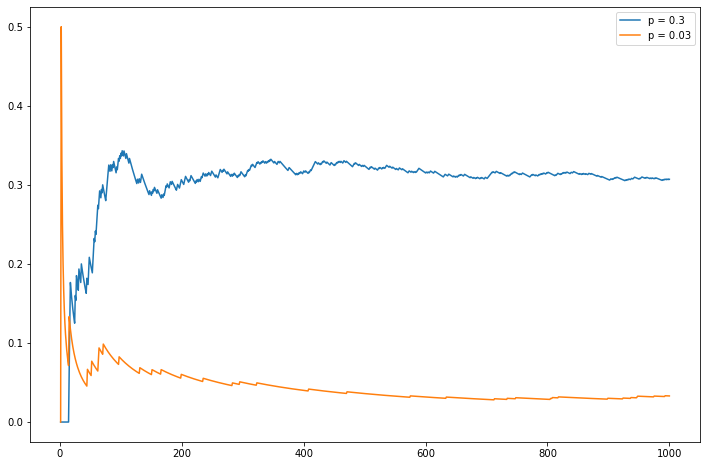
\includegraphics{Figure-02-01}
\end{figure}

\textbf{Exercise 2.10.21 (Computer Experiment)}. Suppose we flip a coin \(n\) times and let \(p\) denote the probability of heads. Let \(X\) be the number of heads. We call \(X\) a binomial random variable which is discussed in the next chapter. Intuition suggests that \(X\) will be close to \(np\). To see if this is true, we can repeat this experiment many times and average the \(X\) values. Carry out a simulation and compare the averages of the \(X\)s to \(np\). Try this for \(p = .3\) and \(n = 10, 100, 1000\).

\begin{python}
import numpy as np
from tqdm.notebook import tqdm

np.random.seed(0)
B = 50000
p = 0.3
X1 = np.empty(B)
X2 = np.empty(B)
X3 = np.empty(B)

for i in tqdm(range(B)):
    x1 = np.where(np.random.uniform(low=0,high=1,size=10)<p,1,0)
    x2 = np.where(np.random.uniform(low=0,high=1,size=100)<p,1,0)
    x3 = np.where(np.random.uniform(low=0,high=1,size=1000)<p,1,0)
    X1[i] = np.sum(x1)
    X2[i] = np.sum(x2)
    X3[i] = np.sum(x3)
\end{python}

\begin{python}
print('X1 mean: %.3f' % X1.mean())
print('X1 np:   %.3f' % (0.3 * 10))
print()
print('X2 mean: %.3f' % X2.mean())
print('X2 np:   %.3f' % (0.3 * 100))
print()
print('X3 mean: %.3f' % X3.mean())
print('X3 np:   %.3f' % (0.3 * 1000))
\end{python}

\begin{console}
X1 mean: 3.010
X1 np:   3.000

X2 mean: 30.013
X2 np:   30.000

X3 mean: 300.104
X3 np:   300.000
\end{console}

\begin{python}
import matplotlib.pyplot as plt

plt.figure(figsize=(12, 8))

ax = plt.subplot(3, 1, 1)
ax.hist(X1, density=True, bins=100, label='histogram', color='C0')
ax.vlines(X1.mean(), ymin=0, ymax=5, label=r'$\overline{X}$', color='C1')
ax.vlines(0.3 * 10, ymin=0, ymax=5, label=r'$np$', color='C2')
ax.legend(loc='upper right')
ax.set_title('n = 10')

ax = plt.subplot(3, 1, 2)
ax.hist(X2, density=True, bins=100, label='histogram', color='C0')
ax.vlines(X2.mean(), ymin=0, ymax=0.5, label=r'$\overline{X}$', color='C1')
ax.vlines(0.3 * 100, ymin=0, ymax=0.5, label=r'$np$', color='C2')
ax.legend(loc='upper right')
ax.set_title('n = 100')

ax = plt.subplot(3, 1, 3)
ax.hist(X3, density=True, bins=100, label='histogram', color='C0')
ax.vlines(X3.mean(), ymin=0, ymax=0.05, label=r'$\overline{X}$', color='C1')
ax.vlines(0.3 * 1000, ymin=0, ymax=0.05, label=r'$np$', color='C2')
ax.legend(loc='upper right')
ax.set_title('n = 1000')

plt.tight_layout()
plt.show()
\end{python}

\begin{figure}[H]
\centering
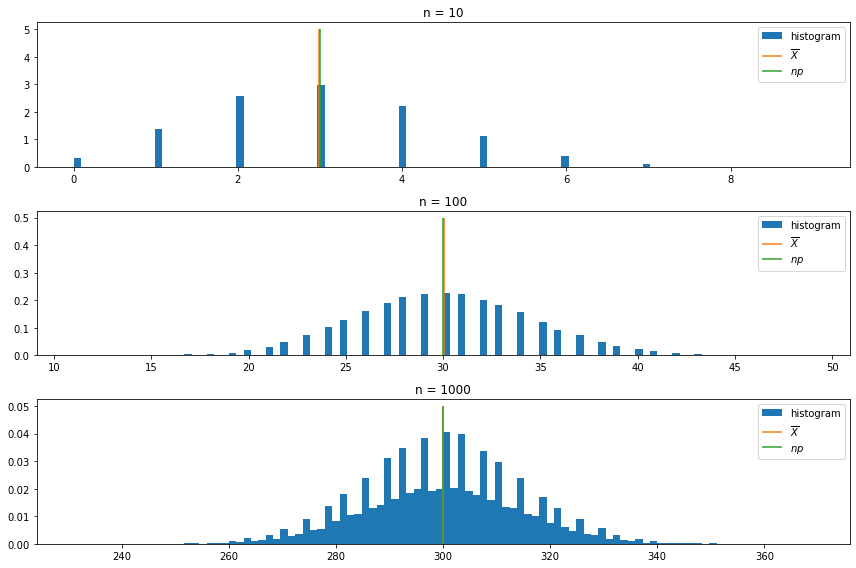
\includegraphics{Figure-02-02}
\end{figure}

\textbf{Exercise 2.10.22 (Computer Experiment)}. Here we will get some experience simulating conditional probabilities. Consider tossing a fair die. Let \(A = \{2, 4, 6\}\) and \(B = \{1, 2, 3, 4\}\). Then \(\mathbb{P}(A) = 1/2\), \(\mathbb{P}(B) = 2/3\) and \(\mathbb{P}(AB) = 1/3\). Since \(\mathbb{P}(AB) = \mathbb{P}(A) \mathbb{P}(B)\), the events \(A\) and \(B\) are independent. Simulate draws from the sample space and verify that \(\hat{P}(AB) = \hat{P}(A) \hat{P}(B)\) where \(\hat{P}\) is the proportion of times an event occurred in the simulation. Now find two events \(A\) and \(B\) that are not independent. Compute \(\hat{P}(A)\), \(\hat{P}(B)\) and \(\hat{P}(AB)\). Compare the calculated values to their theoretical values. Report your results and interpret.

\begin{python}
import numpy as np

np.random.seed(0)

B = 10000
results = np.random.randint(low=1, high=7, size=B)

A_hat = np.isin(results, [2, 4, 6])
B_hat = np.isin(results, [1, 2, 3, 4])
AB_hat = np.isin(results, [2, 4])
\end{python}

\begin{python}
import matplotlib.pyplot as plt

nn = np.arange(1, B + 1)

f, (a0, a1) = plt.subplots(2, 1, gridspec_{k}w={'height_ratios': [3, 1]}, figsize=(12, 8))

a0.plot(nn, np.cumsum(A_hat) / nn, label=r'$\hat{P}(A)$')
a0.plot(nn, np.cumsum(B_hat) / nn, label=r'$\hat{P}(B)$')
a0.plot(nn, np.cumsum(AB_hat) / nn, label=r'$\hat{P}(AB)$')
a0.plot(nn, np.cumsum(A_hat) * np.cumsum(B_hat) / (nn * nn), label=r'$\hat{P}(A) \hat{P}(B)$')
a0.legend(loc='upper right')

a1.plot(nn, np.cumsum(A_hat) * np.cumsum(B_hat) / (nn * nn) - np.cumsum(AB_hat) / nn, 
         label=r'$\hat{P}(A) \hat{P}(B)- \hat{P}(AB)$', color='purple')
a1.legend(loc='upper right')

plt.tight_layout()
plt.show()
\end{python}

\begin{figure}[H]
\centering
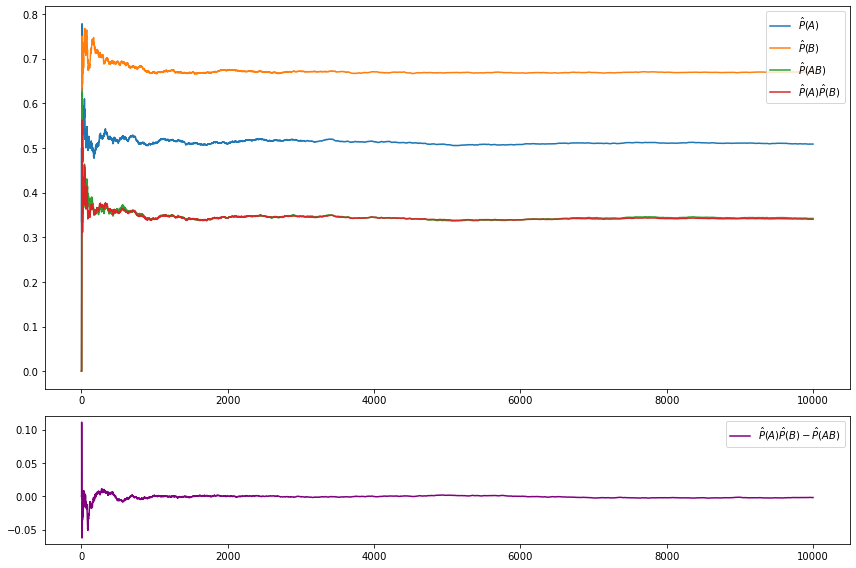
\includegraphics{Figure-02-03}
\end{figure}

For our own choice of non-independent events, let \(A = \{ 2, 4, 6\}\)
and \(B = \{2, 4, 5\}\). Then \(\mathbb{P}(A) = \mathbb{P}(B) = 1/2\)
but \(\mathbb{P}(AB) = 1/3\).

\begin{python}
A_hat = np.isin(results, [2, 4, 6])
B_hat = np.isin(results, [2, 4, 5])
AB_hat = np.isin(results, [2, 4])
\end{python}

\begin{python}
import matplotlib.pyplot as plt

nn = np.arange(1, B + 1)

f, (a0, a1) = plt.subplots(2, 1, gridspec_{k}w={'height_ratios': [3, 1]}, figsize=(12, 8))

a0.plot(nn, np.cumsum(A_hat) / nn, label=r'$\hat{P}(A)$')
a0.plot(nn, np.cumsum(B_hat) / nn, label=r'$\hat{P}(B)$')
a0.plot(nn, np.cumsum(AB_hat) / nn, label=r'$\hat{P}(AB)$')
a0.plot(nn, np.cumsum(A_hat) * np.cumsum(B_hat) / (nn * nn), label=r'$\hat{P}(A) \hat{P}(B)$')
a0.legend(loc='upper right')

a1.plot(nn, np.cumsum(A_hat) * np.cumsum(B_hat) / (nn * nn) - np.cumsum(AB_hat) / nn, 
         label=r'$\hat{P}(A) \hat{P}(B)- \hat{P}(AB)$', color='purple')
a1.legend(loc='upper right')

plt.tight_layout()
plt.show()
\end{python}

\begin{figure}[H]
\centering
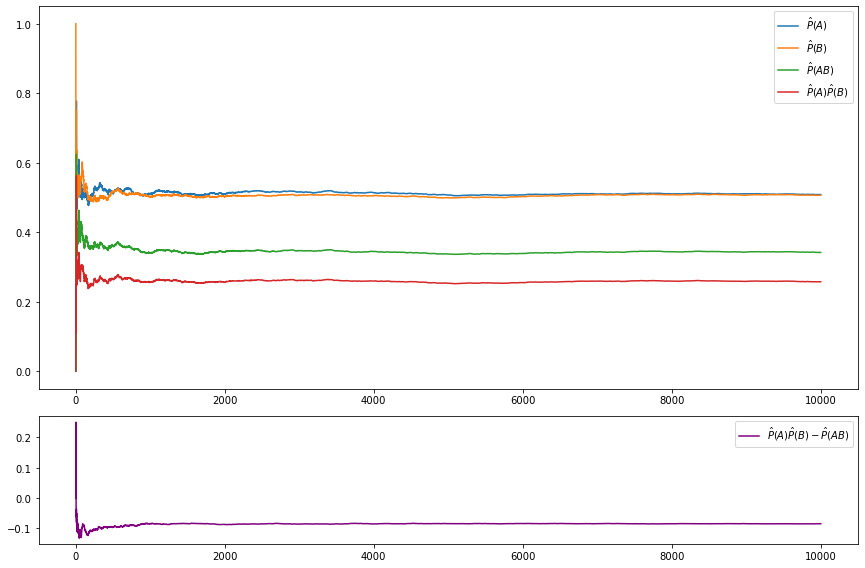
\includegraphics{Figure-02-04}
\end{figure}

As noted, the estimates converges to the theoretical value -- and the
product of the estimates only converge to the estimate of the joint
event in the scenario where the events are independent.

